\documentclass[parskip]{scrartcl}
\usepackage[margin=15mm,landscape]{geometry}
\usepackage{tikz}
 \usetikzlibrary{calc}
 \usetikzlibrary{shapes.geometric}
 \usetikzlibrary{arrows,decorations.pathmorphing,backgrounds,positioning,fit,matrix}
\usepackage{scalefnt}

\begin{document}

%page 1
%%%%%%%%%%%%%%%%%%%%%%%%%%%%%%%%%%%%%%%%%%%%%%%%%%%%%%%%%%%%%%%%%%%%%%%%%%%%
\begin{figure}
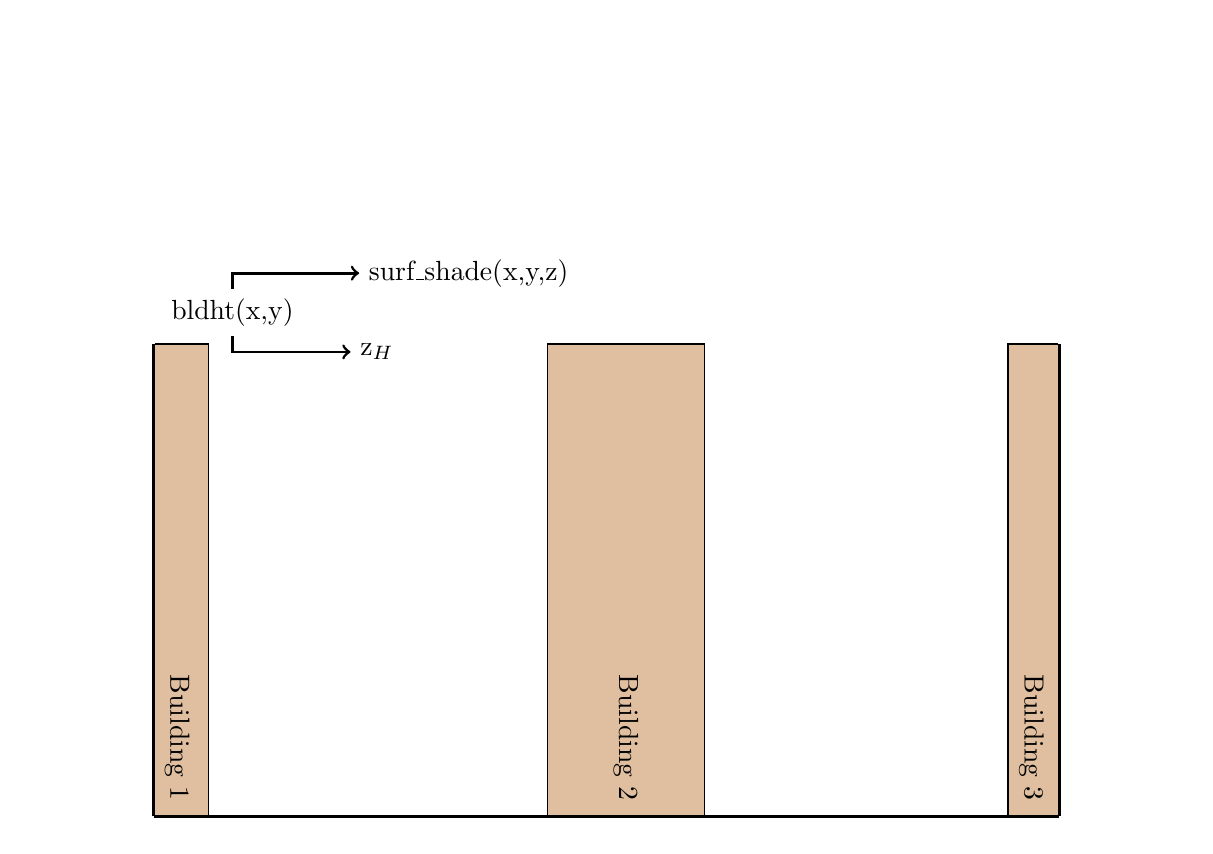
\begin{tikzpicture}

\coordinate (LEFTCORNER) at (0,0);
\coordinate (BUILDING1) at (LEFTCORNER)++(5,0);
\node at (LEFTCORNER) (input) {};
  


%draw building
\node[rectangle,minimum height=6cm,minimum width=2.0cm,fill=brown!50!white,draw=black] at ($(input)+(6,3)$) (BUILDING2) {};
\node[rotate=-90] at ($(input)+(6,1.0)$) {Building 2};

%%%%%%%

%draw building 1 + 3 then clip it at the y-axis
\node[rectangle,minimum height=6cm,minimum width=2.0cm,fill=brown!50!white,draw=black] at ($(input)+(-0.3,3)$) (BUILDING1) {};
\node[rotate=-90] at ($(input)+(0.3,1.0)$) {Building 1};

\node[rectangle,minimum height=6.1cm,minimum width=1.6cm,fill=white!50!white] at ($(input)+(-0.8,3)$) (BUILDING2) {};

\node[rectangle,minimum height=6cm,minimum width=2.0cm,fill=brown!50!white,draw=black] at ($(input)+(11.85,3)$) (BUILDING3) {};
\node[rotate=-90] at ($(input)+(11.15,1.0)$) {Building 3};

\node[rectangle,minimum height=6.1cm,minimum width=1.6cm,fill=white!50!white] at ($(input)+(12.3,3)$) (BUILDING2) {};

\draw[line width=1.0pt] (LEFTCORNER) ++(0,0)  -- ++(11.5,0);
% change this to get rid of the extra y-axis
\draw[line width=1.0pt,white] (LEFTCORNER) ++(0,0)  -- ++(0,10);
\draw[line width=1.0pt,white] (LEFTCORNER) ++(11.5,0) -- ++(0,10);

\draw[line width=1.0pt] (LEFTCORNER) ++(0,0)  -- ++(0,6);
\draw[line width=1.0pt] (LEFTCORNER) ++(11.5,0) -- ++(0,6);

\node[rotate=0] at ($(input)+(1.0,6.4)$) (bldht) {bldht(x,y)};
\node[rotate=0,anchor=west] at ($(bldht)+(1.5,-0.5)$) (zH) {z$_{H}$};
\node[rotate=0] at ($(bldht)+(3.0,0.5)$) (surfshade) { surf\_shade(x,y,z) };
%\draw (bldht) edge[out=0,in=10,->] (zH);
 \draw[arrows=->,line width=1.0pt](bldht) |- (zH);	 
 \draw[arrows=->,line width=1.0pt](bldht) |- (surfshade);	 

    
\end{tikzpicture}
\end{figure}


%page 2
%%%%%%%%%%%%%%%%%%%%%%%%%%%%%%%%%%%%%%%%%%%%%%%%%%%%%%%%%%%%%%%%%%%%%%%%%%%%

\begin{figure}
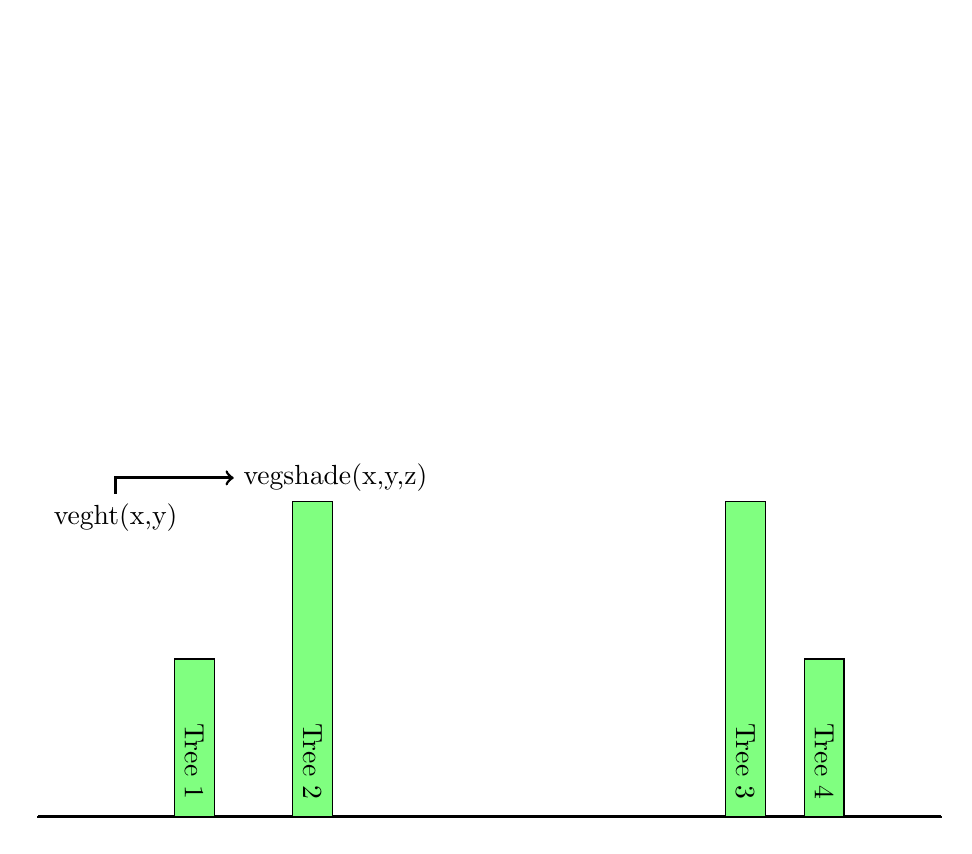
\begin{tikzpicture}

\coordinate (LEFTCORNER) at (0,0);
\coordinate (BUILDING1) at (LEFTCORNER)++(5,0);
\node at (LEFTCORNER) (input) {};
  
% draw x,y
\draw[line width=1.0pt] (LEFTCORNER) ++(0,0)  -- ++(11.5,0);
\draw[line width=1.0pt,white] (LEFTCORNER) ++(0,0)  -- ++(0,10);
\draw[line width=1.0pt,white] (LEFTCORNER) ++(11.5,0) -- ++(0,10);

%%%%%%%%%%%%%%%%%%%
% draw trees
\node[rectangle,minimum height=2cm,minimum width=0.5cm,fill=green!50!white,draw=black] at ($(input)+(2,1)$) (TREE1) {};
\node[rotate=-90] at ($(input)+(2,0.7)$) {Tree 1};
\node[rectangle,minimum height=4cm,minimum width=0.5cm,fill=green!50!white,draw=black] at ($(input)+(3.5,2)$) (TREE2) {};
\node[rotate=-90] at ($(input)+(3.5,0.7)$) {Tree 2};
\node[rectangle,minimum height=4cm,minimum width=0.5cm,fill=green!50!white,draw=black] at ($(input)+(9.0,2)$) (TREE3) {};
\node[rotate=-90] at ($(input)+(9.0,0.7)$) {Tree 3};
\node[rectangle,minimum height=2cm,minimum width=0.5cm,fill=green!50!white,draw=black] at ($(input)+(10.0,1)$) (TREE4) {};
\node[rotate=-90] at ($(input)+(10.0,0.7)$) {Tree 4};

\node[rotate=0] at ($(input)+(1.0,3.8)$) (veght) {veght(x,y)};
\node[rotate=0,anchor=west] at ($(veght)+(1.5,0.5)$) (vegshade) {vegshade(x,y,z)};
 \draw[arrows=->,line width=1.0pt](veght) |- (vegshade);	 

\end{tikzpicture}
\end{figure}


%page 3
%%%%%%%%%%%%%%%%%%%%%%%%%%%%%%%%%%%%%%%%%%%%%%%%%%%%%%%%%%%%%%%%%%%%%%%%%%%%

\begin{figure}
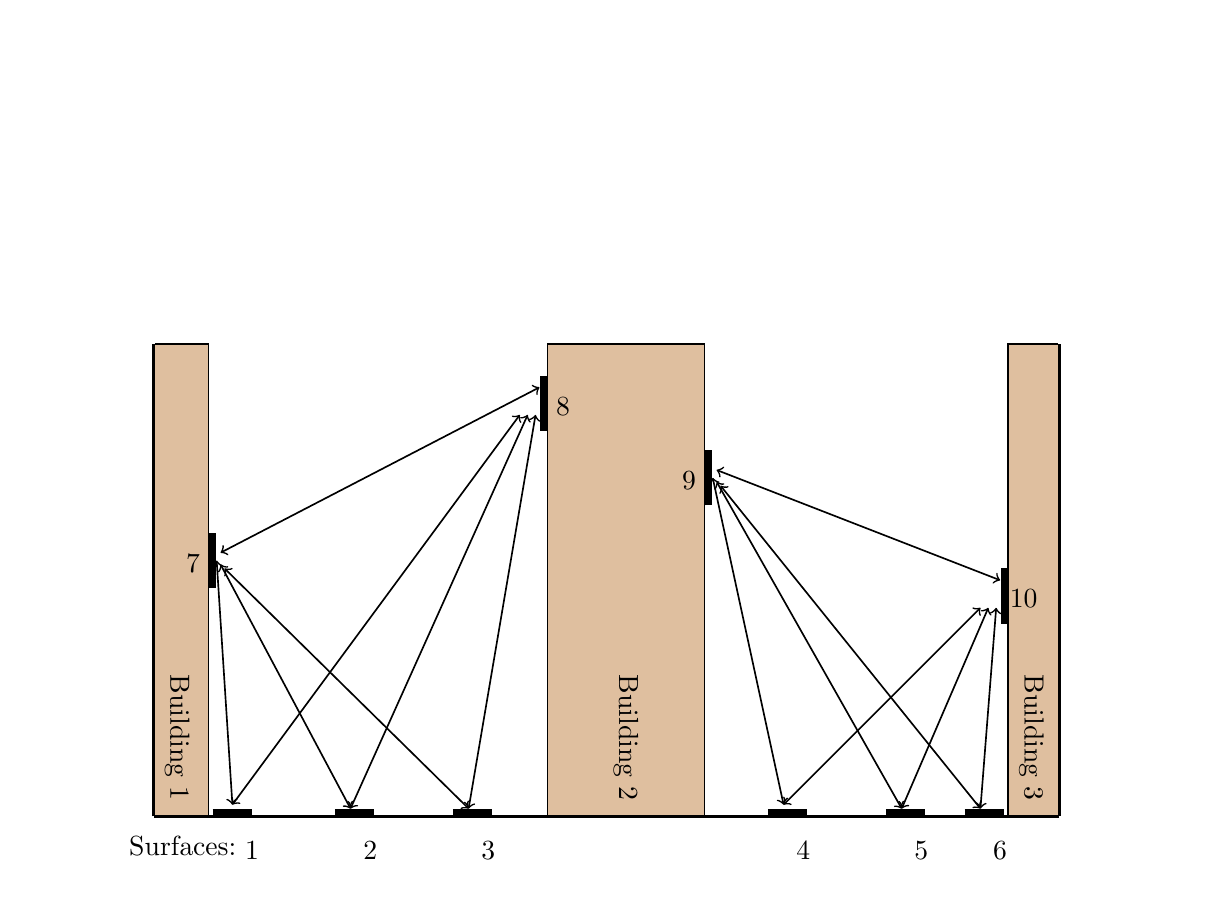
\begin{tikzpicture}

\coordinate (LEFTCORNER) at (0,0);
\coordinate (BUILDING1) at (LEFTCORNER)++(5,0);
\node at (LEFTCORNER) (input) {};
  
% draw x,y
%\draw[line width=1.0pt] (LEFTCORNER) ++(0,0)  -- ++(11.5,0);
%\draw[line width=1.0pt] (LEFTCORNER) ++(0,0)  -- ++(0,10);
%\draw[line width=1.0pt] (LEFTCORNER) ++(11.5,0) -- ++(0,10);

%%%%%%%%%%%%%%%%%%%%%

%draw building
\node[rectangle,minimum height=6cm,minimum width=2.0cm,fill=brown!50!white,draw=black] at ($(input)+(6,3)$) (BUILDING2) {};
\node[rotate=-90] at ($(input)+(6,1.0)$) {Building 2};

%%%%%%%

%draw building 1 + 3 then clip it at the y-axis
\node[rectangle,minimum height=6cm,minimum width=2.0cm,fill=brown!50!white,draw=black] at ($(input)+(-0.3,3)$) (BUILDING1) {};
\node[rotate=-90] at ($(input)+(0.3,1.0)$) {Building 1};

\node[rectangle,minimum height=6.1cm,minimum width=1.6cm,fill=white!50!white] at ($(input)+(-0.8,3)$) (BUILDING2) {};

\node[rectangle,minimum height=6cm,minimum width=2.0cm,fill=brown!50!white,draw=black] at ($(input)+(11.85,3)$) (BUILDING3) {};
\node[rotate=-90] at ($(input)+(11.15,1.0)$) {Building 3};

\node[rectangle,minimum height=6.1cm,minimum width=1.6cm,fill=white!50!white] at ($(input)+(12.3,3)$) (BUILDING2) {};

\draw[line width=1.0pt] (LEFTCORNER) ++(0,0)  -- ++(11.5,0);
%erase the extra y axis
\draw[line width=1.0pt,white] (LEFTCORNER) ++(0,0)  -- ++(0,10);
\draw[line width=1.0pt,white] (LEFTCORNER) ++(11.5,0) -- ++(0,10);

%redraw y-axis by building
\draw[line width=1.0pt] (LEFTCORNER) ++(0,0)  -- ++(0,6);
\draw[line width=1.0pt] (LEFTCORNER) ++(11.5,0) -- ++(0,6);

%%%%%%%%%%%%%%%%%%%
%draw surfaces

\node[rotate=0] at ($(input)+(0.37,-0.37)$) {Surfaces:};

\node[label={[xshift=0.25cm, yshift=-0.8cm]1}] at ($(input)+(1.0,0)$) (SURFACE1) {};
\draw[arrows=-,line width=2.5pt] (SURFACE1)++(-0.25,0.05) -- ++(0.5,0.0) {} ; 

\node[label={[xshift=0.25cm, yshift=-0.8cm]2}] at ($(input)+(2.5,0)$) (SURFACE2) {};
\draw[arrows=-,line width=2.5pt] (SURFACE2)++(-0.2,0.05) -- ++(0.5,0.0) {} ; 

\node[label={[xshift=0.25cm, yshift=-0.8cm]3}] at ($(input)+(4.0,0)$) (SURFACE3) {};
\draw[arrows=-,line width=2.5pt] (SURFACE3)++(-0.2,0.05) -- ++(0.5,0.0) {} ; 

\node[label={[xshift=0.25cm, yshift=-0.8cm]4}] at ($(input)+(8.0,0)$) (SURFACE4) {};
\draw[arrows=-,line width=2.5pt] (SURFACE4)++(-0.2,0.05) -- ++(0.5,0.0) {} ; 

\node[label={[xshift=0.25cm, yshift=-0.8cm]5}] at ($(input)+(9.5,0)$) (SURFACE5) {};
\draw[arrows=-,line width=2.5pt] (SURFACE5)++(-0.2,0.05) -- ++(0.5,0.0) {} ; 

\node[label={[xshift=0.25cm, yshift=-0.8cm]6}] at ($(input)+(10.5,0)$) (SURFACE6) {};
\draw[arrows=-,line width=2.5pt] (SURFACE6)++(-0.2,0.05) -- ++(0.5,0.0) {} ; 

%draw surfaces on building sides
\node[label={[xshift=-0.5cm, yshift=0.4cm]7}] at ($(input)+(1.0,2.45)$) (SURFACE7) {};
\draw[arrows=-,line width=2.5pt] (SURFACE7)++(-0.25,0.45) -- ++(0.0,0.70) {} ; 

\node[label={[xshift=-0.0cm, yshift=0.4cm]8}] at ($(input)+(5.2,4.45)$) (SURFACE8) {};
\draw[arrows=-,line width=2.5pt] (SURFACE8)++(-0.25,0.45) -- ++(0.0,0.70) {} ; 

\node[label={[xshift=-0.5cm, yshift=0.4cm]9}] at ($(input)+(7.3,3.5)$) (SURFACE9) {};
\draw[arrows=-,line width=2.5pt] (SURFACE9)++(-0.25,0.45) -- ++(0.0,0.70) {} ; 

\node[label={[xshift=-0.0cm, yshift=0.4cm]10}] at ($(input)+(11.05,2.0)$) (SURFACE10) {};
\draw[arrows=-,line width=2.5pt] (SURFACE10)++(-0.25,0.45) -- ++(0.0,0.70) {} ; 


%draw arrows between surfaces
\draw[arrows=<->,line width=0.6pt] ($(SURFACE9)+(-0.15,0.9)$) -- ($(SURFACE10)+(-0.3,1.0)$) {} ;

\draw[arrows=<->,line width=0.6pt] ($(SURFACE6)+(-0.0,0.1)$) -- ($(SURFACE10)+(-0.35,0.65)$) {} ;
\draw[arrows=<->,line width=0.6pt] ($(SURFACE5)+(-0.0,0.1)$) -- ($(SURFACE10)+(-0.45,0.65)$) {} ;
\draw[arrows=<->,line width=0.6pt] ($(SURFACE4)+(-0.0,0.15)$) -- ($(SURFACE10)+(-0.55,0.65)$) {} ;

\draw[arrows=<->,line width=0.6pt] ($(SURFACE6)+(-0.0,0.1)$) -- ($(SURFACE9)+(-0.1,0.7)$) {} ;
\draw[arrows=<->,line width=0.6pt] ($(SURFACE5)+(-0.0,0.1)$) -- ($(SURFACE9)+(-0.15,0.75)$) {} ;
\draw[arrows=<->,line width=0.6pt] ($(SURFACE4)+(-0.0,0.15)$) -- ($(SURFACE9)+(-0.2,0.8)$) {} ;

\draw[arrows=<->,line width=0.6pt] ($(SURFACE7)+(-0.15,0.9)$) -- ($(SURFACE8)+(-0.3,1.0)$) {} ;

\draw[arrows=<->,line width=0.6pt] ($(SURFACE3)+(-0.0,0.1)$) -- ($(SURFACE8)+(-0.35,0.65)$) {} ;
\draw[arrows=<->,line width=0.6pt] ($(SURFACE2)+(-0.0,0.1)$) -- ($(SURFACE8)+(-0.45,0.65)$) {} ;
\draw[arrows=<->,line width=0.6pt] ($(SURFACE1)+(-0.0,0.15)$) -- ($(SURFACE8)+(-0.55,0.65)$) {} ;


\draw[arrows=<->,line width=0.6pt] ($(SURFACE3)+(-0.0,0.1)$) -- ($(SURFACE7)+(-0.1,0.7)$) {} ;
\draw[arrows=<->,line width=0.6pt] ($(SURFACE2)+(-0.0,0.1)$) -- ($(SURFACE7)+(-0.15,0.75)$) {} ;
\draw[arrows=<->,line width=0.6pt] ($(SURFACE1)+(-0.0,0.15)$) -- ($(SURFACE7)+(-0.2,0.8)$) {} ;

%%%%%%%%%%%%%%%%%%%%%%
    
\end{tikzpicture}
\end{figure}



%page 4
%%%%%%%%%%%%%%%%%%%%%%%%%%%%%%%%%%%%%%%%%%%%%%%%%%%%%%%%%%%%%%%%%%%%%%%%%%%%

\begin{figure}
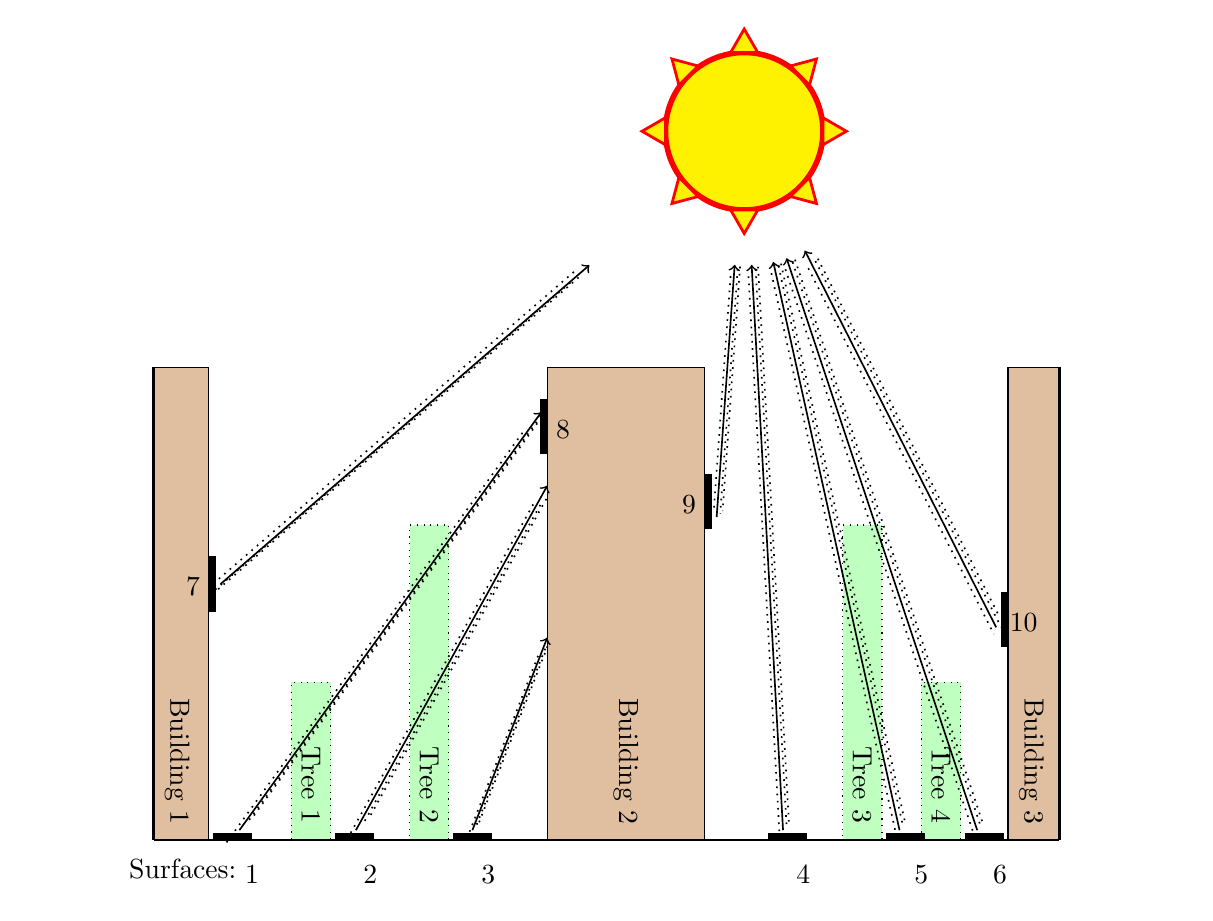
\begin{tikzpicture}

\coordinate (LEFTCORNER) at (0,0);
\coordinate (BUILDING1) at (LEFTCORNER)++(5,0);
\node at (LEFTCORNER) (input) {};


%%%%%%%%%%%%%%%%%%%%%
draw sun
	
\tikzset{
    sunflames/.style={
        line width=1pt,draw=red,fill=yellow,regular polygon, 
        regular polygon sides=3,inner sep=0.07cm
    },
    sunbody/.style={line width=2pt,draw=red,
        fill=yellow,circle,minimum size=2cm
    }
 }
	
\draw (LEFTCORNER)  ++(7.5,9.0)  node[sunbody] (TheSun) {};
\foreach \angle in { 0,45,...,359  }
  {
   \draw [rotate around={\angle:(TheSun.center)}]
      ($(TheSun.center) + (1.1,0)$) node[shape border rotate=\angle-90,sunflames] {};
   }

%%%%%%%%%%%%%%%%%%%
 draw trees

\node[rectangle,minimum height=2cm,minimum width=0.5cm,fill=green!25!white,draw=black,dotted] at ($(input)+(2,1)$) (TREE1) {};
\node[rotate=-90] at ($(input)+(2,0.7)$) {Tree 1};

\node[rectangle,minimum height=4cm,minimum width=0.5cm,fill=green!25!white,draw=black,dotted] at ($(input)+(3.5,2)$) (TREE2) {};
\node[rotate=-90] at ($(input)+(3.5,0.7)$) {Tree 2};

\node[rectangle,minimum height=4cm,minimum width=0.5cm,fill=green!25!white,draw=black,dotted] at ($(input)+(9.0,2)$) (TREE3) {};
\node[rotate=-90] at ($(input)+(9.0,0.7)$) {Tree 3};

\node[rectangle,minimum height=2cm,minimum width=0.5cm,fill=green!25!white,draw=black,dotted] at ($(input)+(10.0,1)$) (TREE4) {};
\node[rotate=-90] at ($(input)+(10.0,0.7)$) {Tree 4};




%draw building
\node[rectangle,minimum height=6cm,minimum width=2.0cm,fill=brown!50!white,draw=black] at ($(input)+(6,3)$) (BUILDING2) {};
\node[rotate=-90] at ($(input)+(6,1.0)$) {Building 2};

%%%%%%%

%draw building 1 + 3 then clip it at the y-axis
\node[rectangle,minimum height=6cm,minimum width=2.0cm,fill=brown!50!white,draw=black] at ($(input)+(-0.3,3)$) (BUILDING1) {};
\node[rotate=-90] at ($(input)+(0.3,1.0)$) {Building 1};

\node[rectangle,minimum height=6.1cm,minimum width=1.6cm,fill=white!50!white] at ($(input)+(-0.8,3)$) (BUILDING2) {};

\node[rectangle,minimum height=6cm,minimum width=2.0cm,fill=brown!50!white,draw=black] at ($(input)+(11.85,3)$) (BUILDING3) {};
\node[rotate=-90] at ($(input)+(11.15,1.0)$) {Building 3};

\node[rectangle,minimum height=6.1cm,minimum width=1.6cm,fill=white!50!white] at ($(input)+(12.3,3)$) (BUILDING2) {};

\draw[line width=1.0pt] (LEFTCORNER) ++(0,0)  -- ++(11.5,0);
%erase extra y-axis
\draw[line width=1.0pt,white] (LEFTCORNER) ++(0,0)  -- ++(0,10);
\draw[line width=1.0pt,white] (LEFTCORNER) ++(11.5,0) -- ++(0,10);
%redraw y-axis by buildings
\draw[line width=1.0pt] (LEFTCORNER) ++(0,0)  -- ++(0,6);
\draw[line width=1.0pt] (LEFTCORNER) ++(11.5,0) -- ++(0,6);



%%%%%%%%%%%%%%%%%%%
draw surfaces

\node[rotate=0] at ($(input)+(0.37,-0.37)$) {Surfaces:};

\node[label={[xshift=0.25cm, yshift=-0.8cm]1}] at ($(input)+(1.0,0)$) (SURFACE1) {};
\draw[arrows=-,line width=2.5pt] (SURFACE1)++(-0.25,0.05) -- ++(0.5,0.0) {} ; 

\node[label={[xshift=0.25cm, yshift=-0.8cm]2}] at ($(input)+(2.5,0)$) (SURFACE2) {};
\draw[arrows=-,line width=2.5pt] (SURFACE2)++(-0.2,0.05) -- ++(0.5,0.0) {} ; 

\node[label={[xshift=0.25cm, yshift=-0.8cm]3}] at ($(input)+(4.0,0)$) (SURFACE3) {};
\draw[arrows=-,line width=2.5pt] (SURFACE3)++(-0.2,0.05) -- ++(0.5,0.0) {} ; 

\node[label={[xshift=0.25cm, yshift=-0.8cm]4}] at ($(input)+(8.0,0)$) (SURFACE4) {};
\draw[arrows=-,line width=2.5pt] (SURFACE4)++(-0.2,0.05) -- ++(0.5,0.0) {} ; 

\node[label={[xshift=0.25cm, yshift=-0.8cm]5}] at ($(input)+(9.5,0)$) (SURFACE5) {};
\draw[arrows=-,line width=2.5pt] (SURFACE5)++(-0.2,0.05) -- ++(0.5,0.0) {} ; 

\node[label={[xshift=0.25cm, yshift=-0.8cm]6}] at ($(input)+(10.5,0)$) (SURFACE6) {};
\draw[arrows=-,line width=2.5pt] (SURFACE6)++(-0.2,0.05) -- ++(0.5,0.0) {} ; 


%draw surfaces on building sides
\node[label={[xshift=-0.5cm, yshift=0.4cm]7}] at ($(input)+(1.0,2.45)$) (SURFACE7) {};
\draw[arrows=-,line width=2.5pt] (SURFACE7)++(-0.25,0.45) -- ++(0.0,0.70) {} ; 

\node[label={[xshift=-0.0cm, yshift=0.4cm]8}] at ($(input)+(5.2,4.45)$) (SURFACE8) {};
\draw[arrows=-,line width=2.5pt] (SURFACE8)++(-0.25,0.45) -- ++(0.0,0.70) {} ; 

\node[label={[xshift=-0.5cm, yshift=0.4cm]9}] at ($(input)+(7.3,3.5)$) (SURFACE9) {};
\draw[arrows=-,line width=2.5pt] (SURFACE9)++(-0.25,0.45) -- ++(0.0,0.70) {} ; 

\node[label={[xshift=-0.0cm, yshift=0.4cm]10}] at ($(input)+(11.05,2.0)$) (SURFACE10) {};
\draw[arrows=-,line width=2.5pt] (SURFACE10)++(-0.25,0.45) -- ++(0.0,0.70) {} ; 
%%%%%%%%%%%%%%%%%%%%%
     
%     
%draw trace rays 
%ray 1
% from surface
\draw[arrows=<-,line width=0.6pt,shorten <=4.4cm,shorten >=0.0cm] (TheSun.center)++(0.0,0.0) -- (SURFACE1) {} ;
\draw[dotted,transform canvas={xshift=-1.2ex,yshift=-1.2ex},arrows=-,line width=0.6pt,shorten <=4.5cm] (TheSun.center)++(0.0,0.0) -- (SURFACE1) {} ;
\draw[dotted,transform canvas={xshift=0.7ex,yshift=0.7ex},arrows=-,line width=0.6pt,shorten <=4.5cm] (TheSun.center)++(0.0,0.0) -- (SURFACE1) {} ;
\draw[dotted,transform canvas={xshift=1.2ex,yshift=1.2ex},arrows=-,line width=0.6pt,shorten <=4.8cm] (TheSun.center)++(0.0,0.0) -- (SURFACE1) {} ;

%ray 2
%from surface
\draw[arrows=<-,line width=0.6pt,shorten <=5.15cm,shorten >=0.0cm] (TheSun.center)++(0.0,0.0) -- (SURFACE2) {} ;
\draw[dotted,transform canvas={xshift=-0.7ex,yshift=-0.7ex},arrows=-,line width=0.6pt,shorten <=5.3cm] (TheSun.center)++(0.0,0.0) -- (SURFACE2) {} ;
\draw[dotted,transform canvas={xshift=0.7ex,yshift=0.7ex},arrows=-,line width=0.6pt,shorten <=5.55cm] (TheSun.center)++(0.0,0.0) -- (SURFACE2) {} ;
\draw[dotted,transform canvas={xshift=1.2ex,yshift=1.2ex},arrows=-,line width=0.6pt,shorten <=5.55cm] (TheSun.center)++(0.0,0.0) -- (SURFACE2) {} ;

%ray 3
\draw[arrows=<-,line width=0.6pt,shorten <=6.9cm] (TheSun.center)++(0.0,0.0) -- (SURFACE3) {} ;
\draw[dotted,transform canvas={xshift=-0.3ex,yshift=-0.3ex},arrows=-,line width=0.6pt,shorten <=7.1cm] (TheSun.center)++(0.0,0.0) -- (SURFACE3) {} ;
\draw[dotted,transform canvas={xshift=0.3ex,yshift=0.3ex},arrows=-,line width=0.6pt,shorten <=7.1cm] (TheSun.center)++(0.0,0.0) -- (SURFACE3) {} ;
\draw[dotted,transform canvas={xshift=0.5ex,yshift=0.5ex},arrows=-,line width=0.6pt,shorten <=7.1cm] (TheSun.center)++(0.0,0.0) -- (SURFACE3) {} ;

%ray 4
\draw[arrows=<-,line width=0.6pt,shorten <=1.7cm] (TheSun.center)++(0.0,0.0) -- (SURFACE4) {} ;
\draw[dotted,transform canvas={xshift=-0.3ex,yshift=-0.3ex},arrows=-,line width=0.6pt,shorten <=1.8cm] (TheSun.center)++(0.0,0.0) -- (SURFACE4) {} ;
\draw[dotted,transform canvas={xshift=0.3ex,yshift=0.3ex},arrows=-,line width=0.6pt,shorten <=1.8cm] (TheSun.center)++(0.0,0.0) -- (SURFACE4) {} ;
\draw[dotted,transform canvas={xshift=0.5ex,yshift=0.5ex},arrows=-,line width=0.6pt,shorten <=1.8cm] (TheSun.center)++(0.0,0.0) -- (SURFACE4) {} ;

%ray 5
%from surface
\draw[arrows=<-,line width=0.6pt,shorten <=1.7cm] (TheSun.center)++(0.0,0.0) -- (SURFACE5) {} ;
\draw[dotted,transform canvas={xshift=-0.3ex,yshift=-0.3ex},arrows=-,line width=0.6pt,shorten <=1.8cm] (TheSun.center)++(0.0,0.0) -- (SURFACE5) {} ;
\draw[dotted,transform canvas={xshift=0.3ex,yshift=0.3ex},arrows=-,line width=0.6pt,shorten <=1.8cm] (TheSun.center)++(0.0,0.0) -- (SURFACE5) {} ;
\draw[dotted,transform canvas={xshift=0.5ex,yshift=0.5ex},arrows=-,line width=0.6pt,shorten <=1.8cm] (TheSun.center)++(0.0,0.0) -- (SURFACE5) {} ;

%ray 6
%from surface
\draw[arrows=<-,line width=0.6pt,shorten <=1.7cm] (TheSun.center)++(0.0,0.0) -- (SURFACE6) {} ;
\draw[dotted,transform canvas={xshift=-0.3ex,yshift=-0.3ex},arrows=-,line width=0.6pt,shorten <=1.8cm] (TheSun.center)++(0.0,0.0) -- (SURFACE6) {} ;
\draw[dotted,transform canvas={xshift=0.3ex,yshift=0.3ex},arrows=-,line width=0.6pt,shorten <=1.8cm] (TheSun.center)++(0.0,0.0) -- (SURFACE6) {} ;
\draw[dotted,transform canvas={xshift=0.5ex,yshift=0.5ex},arrows=-,line width=0.6pt,shorten <=1.8cm] (TheSun.center)++(0.0,0.0) -- (SURFACE6) {} ;


%ray 7
%from surface
\draw[arrows=<-,line width=0.6pt,shorten <=2.6cm] (TheSun.center)++(0.0,0.0) -- ($(SURFACE7)+(-0.15,0.8)$) {} ;
\draw[dotted,transform canvas={xshift=-1.9ex,yshift=-1.9ex},arrows=-,line width=0.6pt,shorten <=2.4cm,shorten >=0.3cm] (TheSun.center)++(0.0,0.0) -- ($(SURFACE7)+(-0.15,0.8)$) {} ;
\draw[dotted,transform canvas={xshift=-0.6ex,yshift=-0.6ex},arrows=-,line width=0.6pt,shorten <=2.8cm] (TheSun.center)++(0.0,0.0) -- ($(SURFACE7)+(-0.15,0.8)$) {} ;
\draw[dotted,transform canvas={xshift=-0.3ex,yshift=0.3ex},arrows=-,line width=0.6pt,shorten <=2.8cm] (TheSun.center)++(0.0,0.0) -- ($(SURFACE7)+(-0.15,0.8)$) {} ;

%ray 9
%from surface
\draw[arrows=<-,line width=0.6pt,shorten <=1.7cm] (TheSun.center)++(0.0,0.0) -- ($(SURFACE9)+(-0.15,0.6)$) {} ;
\draw[dotted,transform canvas={xshift=-0.3ex,yshift=-0.3ex},arrows=-,line width=0.6pt,shorten <=1.8cm,shorten >=0.15cm] (TheSun.center)++(0.0,0.0) -- ($(SURFACE9)+(-0.15,0.6)$) {} ;
\draw[dotted,transform canvas={xshift=0.3ex,yshift=0.3ex},arrows=-,line width=0.6pt,shorten <=1.8cm] (TheSun.center)++(0.0,0.0) -- ($(SURFACE9)+(-0.15,0.6)$) {} ;
\draw[dotted,transform canvas={xshift=0.5ex,yshift=0.5ex},arrows=-,line width=0.6pt,shorten <=1.8cm] (TheSun.center)++(0.0,0.0) -- ($(SURFACE9)+(-0.15,0.6)$) {} ;

%ray 10
%from surface
\draw[arrows=<-,line width=0.6pt,shorten <=1.7cm] (TheSun.center)++(0.0,0.0) -- ($(SURFACE10)+(-0.35,0.7)$) {} ;
\draw[dotted,transform canvas={xshift=-0.3ex,yshift=-0.3ex},arrows=-,line width=0.6pt,shorten <=1.9cm, shorten >=0.6cm] (TheSun.center)++(0.0,0.0) -- (SURFACE10) {} ;
\draw[dotted,transform canvas={xshift=0.3ex,yshift=0.3ex},arrows=-,line width=0.6pt,shorten <=1.9cm, shorten >=0.6cm] (TheSun.center)++(0.0,0.0) -- (SURFACE10) {} ;
\draw[dotted,transform canvas={xshift=0.5ex,yshift=0.5ex},arrows=-,line width=0.6pt,shorten <=1.9cm, shorten >=0.7cm] (TheSun.center)++(0.0,0.0) -- (SURFACE10) {} ;

%%%%%%%%%%%%%%%%%%%%%%%%%%%%%%%%%%%%%%%%%%%%%%

    
\end{tikzpicture}
\end{figure}
















\begin{figure}
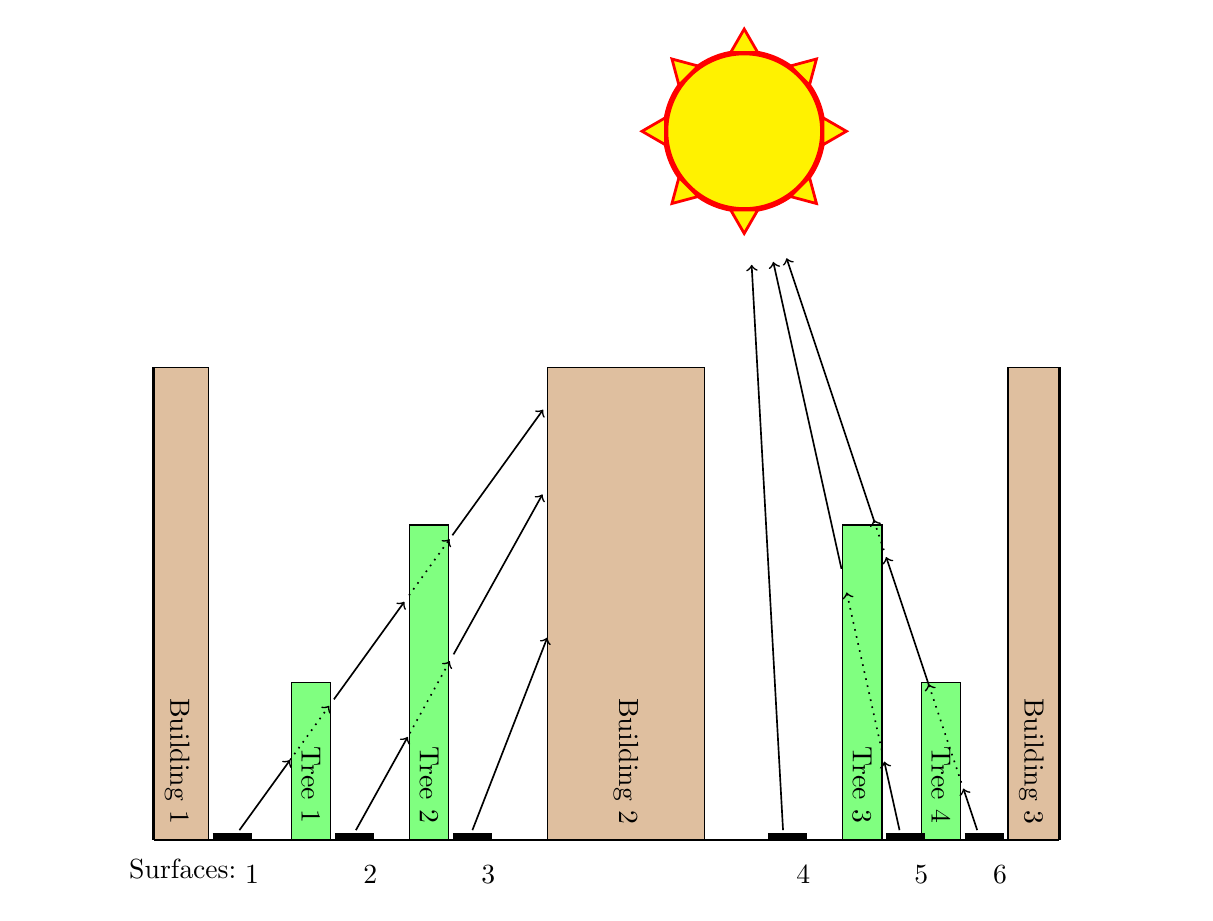
\begin{tikzpicture}



\coordinate (LEFTCORNER) at (0,0);
%\coordinate (TREE1) at (LEFTCORNER)++(2,0);
\coordinate (BUILDING1) at (LEFTCORNER)++(5,0);
\node at (LEFTCORNER) (input) {};
  


%%%%%%%%%%%%%%%%%%%%%
%draw sun
	
\tikzset{
    sunflames/.style={
        line width=1pt,draw=red,fill=yellow,regular polygon, 
        regular polygon sides=3,inner sep=0.07cm
    },
    sunbody/.style={line width=2pt,draw=red,
        fill=yellow,circle,minimum size=2cm
    }
 }
	
\draw (LEFTCORNER)  ++(7.5,9.0)  node[sunbody] (TheSun) {};
\foreach \angle in { 0,45,...,359  }
  {
   \draw [rotate around={\angle:(TheSun.center)}]
      ($(TheSun.center) + (1.1,0)$) node[shape border rotate=\angle-90,sunflames] {};
   }

%%%%%%%%%%%%%%%%%%%
% draw trees
%\fill[green!50!white, draw=black] (LEFTCORNER)++(2,0) rectangle (2.5,3);
\node[rectangle,minimum height=2cm,minimum width=0.5cm,fill=green!50!white,draw=black] at ($(input)+(2,1)$) (TREE1) {};
\node[rotate=-90] at ($(input)+(2,0.7)$) {Tree 1};
%\fill[green!50!white, draw=black] (LEFTCORNER)++(4,0) rectangle (4.5,4);
\node[rectangle,minimum height=4cm,minimum width=0.5cm,fill=green!50!white,draw=black] at ($(input)+(3.5,2)$) (TREE2) {};
\node[rotate=-90] at ($(input)+(3.5,0.7)$) {Tree 2};
%\fill[green!50!white, draw=black] (LEFTCORNER)++(8,0) rectangle (8.5,3);
\node[rectangle,minimum height=4cm,minimum width=0.5cm,fill=green!50!white,draw=black] at ($(input)+(9.0,2)$) (TREE3) {};
\node[rotate=-90] at ($(input)+(9.0,0.7)$) {Tree 3};
%\fill[green!50!white, draw=black] (LEFTCORNER)++(9,0) rectangle (9.5,4);
\node[rectangle,minimum height=2cm,minimum width=0.5cm,fill=green!50!white,draw=black] at ($(input)+(10.0,1)$) (TREE4) {};
\node[rotate=-90] at ($(input)+(10.0,0.7)$) {Tree 4};

%draw building
%\fill[brown!50!white, draw=black] (BUILDING1)++(5,0) rectangle (7,6);
\node[rectangle,minimum height=6cm,minimum width=2.0cm,fill=brown!50!white,draw=black] at ($(input)+(6,3)$) (BUILDING2) {};
\node[rotate=-90] at ($(input)+(6,1.0)$) {Building 2};

%%%%%%%

%draw building 1 + 3 then clip it at the y-axis
\node[rectangle,minimum height=6cm,minimum width=2.0cm,fill=brown!50!white,draw=black] at ($(input)+(-0.3,3)$) (BUILDING1) {};
\node[rotate=-90] at ($(input)+(0.3,1.0)$) {Building 1};

\node[rectangle,minimum height=6.1cm,minimum width=1.6cm,fill=white!50!white] at ($(input)+(-0.8,3)$) (BUILDING2) {};

\node[rectangle,minimum height=6cm,minimum width=2.0cm,fill=brown!50!white,draw=black] at ($(input)+(11.85,3)$) (BUILDING3) {};
\node[rotate=-90] at ($(input)+(11.15,1.0)$) {Building 3};

\node[rectangle,minimum height=6.1cm,minimum width=1.6cm,fill=white!50!white] at ($(input)+(12.3,3)$) (BUILDING2) {};

\draw[line width=1.0pt] (LEFTCORNER) ++(0,0)  -- ++(11.5,0);
%erase extra y-axis
\draw[line width=1.0pt,white] (LEFTCORNER) ++(0,0)  -- ++(0,10);
\draw[line width=1.0pt,white] (LEFTCORNER) ++(11.5,0) -- ++(0,10);
%redraw needed y-axis
\draw[line width=1.0pt] (LEFTCORNER) ++(0,0)  -- ++(0,6);
\draw[line width=1.0pt] (LEFTCORNER) ++(11.5,0) -- ++(0,6);

%%%%%%%%%%%%%%%%%%%%
%draw surfaces

\node[rotate=0] at ($(input)+(0.37,-0.37)$) {Surfaces:};

\node[label={[xshift=0.25cm, yshift=-0.8cm]1}] at ($(input)+(1.0,0)$) (SURFACE1) {};
\draw[arrows=-,line width=2.5pt] (SURFACE1)++(-0.25,0.05) -- ++(0.5,0.0) {} ; 

\node[label={[xshift=0.25cm, yshift=-0.8cm]2}] at ($(input)+(2.5,0)$) (SURFACE2) {};
\draw[arrows=-,line width=2.5pt] (SURFACE2)++(-0.2,0.05) -- ++(0.5,0.0) {} ; 

\node[label={[xshift=0.25cm, yshift=-0.8cm]3}] at ($(input)+(4.0,0)$) (SURFACE3) {};
\draw[arrows=-,line width=2.5pt] (SURFACE3)++(-0.2,0.05) -- ++(0.5,0.0) {} ; 

\node[label={[xshift=0.25cm, yshift=-0.8cm]4}] at ($(input)+(8.0,0)$) (SURFACE4) {};
\draw[arrows=-,line width=2.5pt] (SURFACE4)++(-0.2,0.05) -- ++(0.5,0.0) {} ; 

\node[label={[xshift=0.25cm, yshift=-0.8cm]5}] at ($(input)+(9.5,0)$) (SURFACE5) {};
\draw[arrows=-,line width=2.5pt] (SURFACE5)++(-0.2,0.05) -- ++(0.5,0.0) {} ; 

\node[label={[xshift=0.25cm, yshift=-0.8cm]6}] at ($(input)+(10.5,0)$) (SURFACE6) {};
\draw[arrows=-,line width=2.5pt] (SURFACE6)++(-0.2,0.05) -- ++(0.5,0.0) {} ; 
%%%%%%%%%%%%%%%%%%%%%%%
     
     
%draw trace rays 
%ray 1
% from surface
\draw[arrows=<-,line width=0.6pt,shorten <=9.85cm,shorten >=0.0cm] (TheSun.center)++(0.0,0.0) -- (SURFACE1) {} ;
%through tree
\draw[dotted,arrows=-<,line width=0.6pt,shorten <=9.85cm,shorten >=1.87cm] (TheSun.center)++(0.0,0.0) -- (SURFACE1) {} ;
%up to 2nd tree
\draw[arrows=-<,line width=0.6pt,shorten <=8.9cm,shorten >=3.50cm] (TheSun.center)++(0.0,0.0) -- (SURFACE1) {} ;
%through 2nd tree
\draw[dotted,arrows=-<,line width=0.6pt,shorten <=7.27cm,shorten >=4.48cm] (TheSun.center)++(0.0,0.0) -- (SURFACE1) {} ;
%up to building
\draw[arrows=-<,line width=0.6pt,shorten <=6.33cm,shorten >=6.51cm] (TheSun.center)++(0.0,0.0) -- (SURFACE1) {} ;


%ray 2
%from surface
\draw[arrows=<-,line width=0.6pt,shorten <=8.80cm,shorten >=0.0cm] (TheSun.center)++(0.0,0.0) -- (SURFACE2) {} ;
%through tree
\draw[dotted,arrows=<-,line width=0.6pt,shorten <=7.7cm,shorten >=1.4cm] (TheSun.center)++(0.0,0.0) -- (SURFACE2) {} ;
%to building
\draw[arrows=-<,line width=0.6pt,shorten <=7.6cm,shorten >=4.8cm] (TheSun.center)++(0.0,0.0) -- (SURFACE2) {} ;

%ray 3
\draw[arrows=<-,line width=0.6pt,shorten <=6.9cm] (TheSun.center)++(0.0,0.0) -- (SURFACE3) {} ;

%ray 4
\draw[arrows=<-,line width=0.6pt,shorten <=1.7cm] (TheSun.center)++(0.0,0.0) -- (SURFACE4) {} ;

%ray 5
%from surface
\draw[arrows=<-,line width=0.6pt,shorten <=8.2cm] (TheSun.center)++(0.0,0.0) -- (SURFACE5) {} ;
%through tree
\draw[dotted,arrows=<-,line width=0.6pt,shorten <=6.0cm,shorten >=1.0cm] (TheSun.center)++(0.0,0.0) -- (SURFACE5) {} ;
%to sun
\draw[arrows=<-,line width=0.6pt,shorten <=1.7cm,shorten >=3.4cm] (TheSun.center)++(0.0,0.0) -- (SURFACE5) {} ;

%ray 6
%from surface
\draw[arrows=<-,line width=0.6pt,shorten <=8.8cm] (TheSun.center)++(0.0,0.0) -- (SURFACE6) {} ;
%through tree
\draw[dotted,arrows=<-,line width=0.6pt,shorten <=7.40cm,shorten >=0.6cm] (TheSun.center)++(0.0,0.0) -- (SURFACE6) {} ;
%to 2nd tree
\draw[arrows=<-,line width=0.6pt,shorten <=5.7cm,shorten >=1.95cm] (TheSun.center)++(0.0,0.0) -- (SURFACE6) {} ; 
%through 2nd tree
\draw[dotted,arrows=<-,line width=0.6pt,shorten <=5.2cm,shorten >=3.75cm] (TheSun.center)++(0.0,0.0) -- (SURFACE6) {} ; 
%to sun
\draw[arrows=<-,line width=0.6pt,shorten <=1.7cm,shorten >=4.14cm] (TheSun.center)++(0.0,0.0) -- (SURFACE6) {} ; 
 
 


%%%%%%%%%%%%%%%%%%%%%%%%%%%%%%%%%%%%%%%%%%%%%%

    
\end{tikzpicture}
\end{figure}
















\begin{figure}
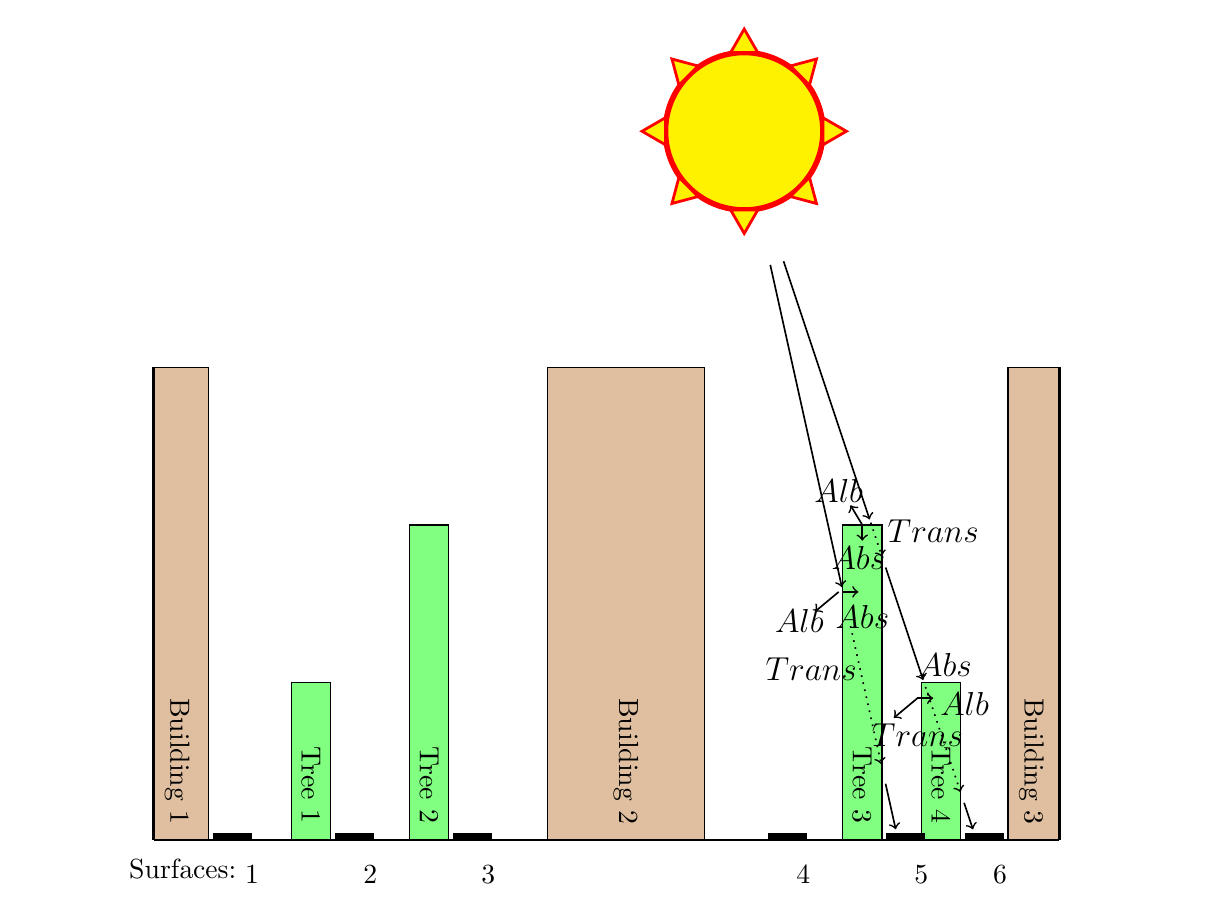
\begin{tikzpicture}



\coordinate (LEFTCORNER) at (0,0);
%\coordinate (TREE1) at (LEFTCORNER)++(2,0);
\coordinate (BUILDING1) at (LEFTCORNER)++(5,0);
\node at (LEFTCORNER) (input) {};
  
% draw x,y
%\draw[line width=1.0pt] (LEFTCORNER) ++(0,0)  -- ++(11.5,0);
%\draw[line width=1.0pt] (LEFTCORNER) ++(0,0)  -- ++(0,10);
%\draw[line width=1.0pt] (LEFTCORNER) ++(11.5,0) -- ++(0,10);

%%%%%%%%%%%%%%%%%%%%%
%draw sun
	
\tikzset{
    sunflames/.style={
        line width=1pt,draw=red,fill=yellow,regular polygon, 
        regular polygon sides=3,inner sep=0.07cm
    },
    sunbody/.style={line width=2pt,draw=red,
        fill=yellow,circle,minimum size=2cm
    }
 }
	
\draw (LEFTCORNER)  ++(7.5,9.0)  node[sunbody] (TheSun) {};
\foreach \angle in { 0,45,...,359  }
  {
   \draw [rotate around={\angle:(TheSun.center)}]
      ($(TheSun.center) + (1.1,0)$) node[shape border rotate=\angle-90,sunflames] {};
   }

%%%%%%%%%%%%%%%%%%%
% draw trees
%\fill[green!50!white, draw=black] (LEFTCORNER)++(2,0) rectangle (2.5,3);
\node[rectangle,minimum height=2cm,minimum width=0.5cm,fill=green!50!white,draw=black] at ($(input)+(2,1)$) (TREE1) {};
\node[rotate=-90] at ($(input)+(2,0.7)$) {Tree 1};
%\fill[green!50!white, draw=black] (LEFTCORNER)++(4,0) rectangle (4.5,4);
\node[rectangle,minimum height=4cm,minimum width=0.5cm,fill=green!50!white,draw=black] at ($(input)+(3.5,2)$) (TREE2) {};
\node[rotate=-90] at ($(input)+(3.5,0.7)$) {Tree 2};
%\fill[green!50!white, draw=black] (LEFTCORNER)++(8,0) rectangle (8.5,3);
\node[rectangle,minimum height=4cm,minimum width=0.5cm,fill=green!50!white,draw=black] at ($(input)+(9.0,2)$) (TREE3) {};
\node[rotate=-90] at ($(input)+(9.0,0.7)$) {Tree 3};
%\fill[green!50!white, draw=black] (LEFTCORNER)++(9,0) rectangle (9.5,4);
\node[rectangle,minimum height=2cm,minimum width=0.5cm,fill=green!50!white,draw=black] at ($(input)+(10.0,1)$) (TREE4) {};
\node[rotate=-90] at ($(input)+(10.0,0.7)$) {Tree 4};

%draw building
%\fill[brown!50!white, draw=black] (BUILDING1)++(5,0) rectangle (7,6);
\node[rectangle,minimum height=6cm,minimum width=2.0cm,fill=brown!50!white,draw=black] at ($(input)+(6,3)$) (BUILDING2) {};
\node[rotate=-90] at ($(input)+(6,1.0)$) {Building 2};

%%%%%%%

%draw building 1 + 3 then clip it at the y-axis
\node[rectangle,minimum height=6cm,minimum width=2.0cm,fill=brown!50!white,draw=black] at ($(input)+(-0.3,3)$) (BUILDING1) {};
\node[rotate=-90] at ($(input)+(0.3,1.0)$) {Building 1};

\node[rectangle,minimum height=6.1cm,minimum width=1.6cm,fill=white!50!white] at ($(input)+(-0.8,3)$) (BUILDING2) {};

\node[rectangle,minimum height=6cm,minimum width=2.0cm,fill=brown!50!white,draw=black] at ($(input)+(11.85,3)$) (BUILDING3) {};
\node[rotate=-90] at ($(input)+(11.15,1.0)$) {Building 3};

\node[rectangle,minimum height=6.1cm,minimum width=1.6cm,fill=white!50!white] at ($(input)+(12.3,3)$) (BUILDING2) {};

\draw[line width=1.0pt] (LEFTCORNER) ++(0,0)  -- ++(11.5,0);
\draw[line width=1.0pt,white] (LEFTCORNER) ++(0,0)  -- ++(0,10);
\draw[line width=1.0pt,white] (LEFTCORNER) ++(11.5,0) -- ++(0,10);
\draw[line width=1.0pt] (LEFTCORNER) ++(0,0)  -- ++(0,6);
\draw[line width=1.0pt] (LEFTCORNER) ++(11.5,0) -- ++(0,6);

%%%%%%%%%%%%%%%%%%%%
%draw surfaces

\node[rotate=0] at ($(input)+(0.37,-0.37)$) {Surfaces:};

\node[label={[xshift=0.25cm, yshift=-0.8cm]1}] at ($(input)+(1.0,0)$) (SURFACE1) {};
\draw[arrows=-,line width=2.5pt] (SURFACE1)++(-0.25,0.05) -- ++(0.5,0.0) {} ; 

\node[label={[xshift=0.25cm, yshift=-0.8cm]2}] at ($(input)+(2.5,0)$) (SURFACE2) {};
\draw[arrows=-,line width=2.5pt] (SURFACE2)++(-0.2,0.05) -- ++(0.5,0.0) {} ; 

\node[label={[xshift=0.25cm, yshift=-0.8cm]3}] at ($(input)+(4.0,0)$) (SURFACE3) {};
\draw[arrows=-,line width=2.5pt] (SURFACE3)++(-0.2,0.05) -- ++(0.5,0.0) {} ; 

\node[label={[xshift=0.25cm, yshift=-0.8cm]4}] at ($(input)+(8.0,0)$) (SURFACE4) {};
\draw[arrows=-,line width=2.5pt] (SURFACE4)++(-0.2,0.05) -- ++(0.5,0.0) {} ; 

\node[label={[xshift=0.25cm, yshift=-0.8cm]5}] at ($(input)+(9.5,0)$) (SURFACE5) {};
\draw[arrows=-,line width=2.5pt] (SURFACE5)++(-0.2,0.05) -- ++(0.5,0.0) {} ; 

\node[label={[xshift=0.25cm, yshift=-0.8cm]6}] at ($(input)+(10.5,0)$) (SURFACE6) {};
\draw[arrows=-,line width=2.5pt] (SURFACE6)++(-0.2,0.05) -- ++(0.5,0.0) {} ; 
%%%%%%%%%%%%%%%%%%%%%%%
     
     
%%draw trace rays 

%%ray 4
%\draw[arrows=<-,line width=0.6pt,shorten <=1.7cm] (TheSun.center)++(0.0,0.0) -- (SURFACE4) {} ;

\tikzset{fontscale/.style = {font=\relsize{#1}}
    }

%ray 5
%from surface
\scalefont{0.5}
%\draw[arrows=<-,line width=0.6pt,shorten <=8.2cm] (TheSun.center)++(0.0,0.0) -- (SURFACE5) {} ;
%through tree
%\draw[dotted,arrows=<-,line width=0.6pt,shorten <=6.0cm,shorten >=1.0cm] (TheSun.center)++(0.0,0.0) -- (SURFACE5) {} ;
%and reflection/transmission arrows/labels
\draw[arrows=->,line width=0.6pt,black] (TheSun.center)++(1.50,-5.00) -- ++(-0.15,0.25) node[label={[xshift=-0.15cm, yshift=-0.15cm]\bfseries \large$Alb$}] {} ;	
\draw[arrows=->,line width=0.6pt,black] (TheSun.center)++(1.50,-5.00) -- ++(-0.0,-0.2) node[label={[xshift=-0.05cm, yshift=-0.55cm]\bfseries \large$Abs$}] {} ;	
\draw[line width=0.6pt,black] (TheSun.center)++(1.50,-5.00) -- ++(0.0,0.0) node[label={[xshift=0.90cm, yshift=-0.40cm]\bfseries \large$Trans$}] {} ;
%to sun
%\draw[arrows=<-,line width=0.6pt,shorten <=1.7cm,shorten >=3.4cm] (TheSun.center)++(0.0,0.0) -- (SURFACE5) {} ;

%and reflection/transmission arrows/labels
\draw[arrows=->,line width=0.6pt,black] (TheSun.center)++(1.20,-5.85) -- ++(-0.3,-0.25) node[label={[xshift=-0.20cm, yshift=-0.45cm]\bfseries \large$Alb$}] {} ;	
\draw[arrows=->,line width=0.6pt,black] (TheSun.center)++(1.25,-5.85) -- ++(0.2,0.0) node[label={[xshift=0.05cm, yshift=-0.65cm]\bfseries \large$Abs$}] {} ;	
\draw[line width=0.6pt,black] (TheSun.center)++(1.25,-5.85) -- ++(0.0,0.0) node[label={[xshift=-0.40cm, yshift=-1.30cm]\bfseries \large$Trans$}] {} ;		


%and reflection/transmission arrows/labels
\draw[arrows=->,line width=0.6pt,black] (TheSun.center)++(2.20,-7.20) -- ++(-0.3,-0.25) node[label={[xshift=0.90cm, yshift=-0.15cm]\bfseries \large$Alb$}] {} ;	
\draw[arrows=->,line width=0.6pt,black] (TheSun.center)++(2.20,-7.20) -- ++(0.2,0.0) node[label={[xshift=0.15cm, yshift=0.10cm]\bfseries \large$Abs$}] {} ;	
\draw[line width=0.6pt,black] (TheSun.center)++(2.20,-7.20) -- ++(0.0,0.0) node[label={[xshift=-0.00cm, yshift=-0.80cm]\bfseries \large$Trans$}] {} ;		
 
 %  \bfseries \large 

%ray 5
%from surface
\draw[transform canvas={xshift=-0.5ex,yshift=-0.5ex},arrows=->,line width=0.6pt,shorten <=8.45cm,shorten >=0.05cm,black] (TheSun.center)++(0.0,0.0) -- (SURFACE5) {} ;
%through tree
\draw[transform canvas={xshift=-0.5ex,yshift=-0.5ex},dotted,arrows=->,line width=0.6pt,shorten <=6.4cm,shorten >=0.9cm,black] (TheSun.center)++(0.0,0.0) -- (SURFACE5) {} ;
%to sun
\draw[transform canvas={xshift=-0.5ex,yshift=-0.5ex},arrows=->,line width=0.6pt,shorten <=1.7cm,shorten >=3.2cm,black] (TheSun.center)++(0.0,0.0) -- (SURFACE5) {} ;

%ray 6
%from surface
\draw[transform canvas={xshift=-0.5ex,yshift=-0.5ex},arrows=->,line width=0.6pt,shorten <=8.95cm,shorten >=0.05cm,black] (TheSun.center)++(0.0,0.0) -- (SURFACE6) {} ;
%through tree
\draw[transform canvas={xshift=-0.5ex,yshift=-0.5ex},dotted,arrows=->,line width=0.6pt,shorten <=7.40cm,shorten >=0.55cm,black] (TheSun.center)++(0.0,0.0) -- (SURFACE6) {} ;
%to 2nd tree
\draw[transform canvas={xshift=-0.5ex,yshift=-0.5ex},arrows=->,line width=0.6pt,shorten <=5.8cm,shorten >=2.05cm,black] (TheSun.center)++(0.0,0.0) -- (SURFACE6) {} ; 
%through 2nd tree
\draw[transform canvas={xshift=-0.5ex,yshift=-0.5ex},dotted,arrows=->,line width=0.6pt,shorten <=5.2cm,shorten >=3.7cm,black] (TheSun.center)++(0.0,0.0) -- (SURFACE6) {} ; 
%to sun
\draw[transform canvas={xshift=-0.5ex,yshift=-0.5ex},arrows=->,line width=0.6pt,shorten <=1.7cm,shorten >=4.2cm,black] (TheSun.center)++(0.0,0.0) -- (SURFACE6) {} ; 
% 



%%%%%%%%%%%%%%%%%%%%%%%%%%%%%%%%%%%%%%%%%%%%%%

    
\end{tikzpicture}
\end{figure}










\end{document}